Para asegurar una implementación correcta del algoritmo QAOA primero se aplica a un problema presentado en la página web de Qiskit~\cite{qiskit_tutorial_antiguo}.
Este problema consiste en resolver MAX-CUT para el \textit{grafo~\ref{fig:4-qiskit grafo}}, que consiste en, asignando un valor 0 o 1 a cada nodo maximizar la cantidad de aristas entre nodos de distinto valor.

\begin{figure}[htbp]{fig:4-qiskit grafo}{Grafo obtenido de\textit{~\cite{qiskit_tutorial_antiguo}}}
  \centering
  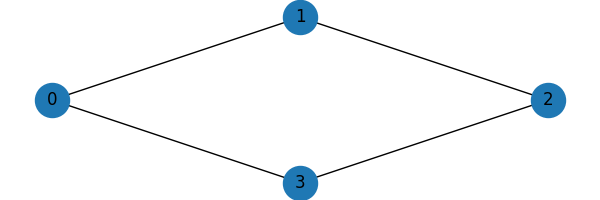
\includegraphics[scale=0.75]{qiskit-grafo/qiskit-grafo.png}
\end{figure}

Se parte de este caso por tratarse de uno sencillo. Esto es porque la cantidad de qubits es pequeña y no existen restricciones en este problema, por lo que el espacio de estados válidos disponibles es de $2^n$, siendo \textit{n} el número de qubits del sistema. Estas condiciones hacen que el algoritmo trabaje sobre un circuito pequeño, lo que reduce el ruido y facilita su implementación.

\begin{itemize}
\item \textbf{Formulación:} \\
  Sea $G = (V, E)$ el grafo de la \textit{figura~\ref{fig:4-qiskit grafo}}, con $V = [0, 1, 2, 3]$ y $E = [(0, 1), (1, 2), (2, 3), (0, 3)]$ los nodos y aristas de G respectivamente

\item \textbf{Objetivo:} \\
  \begin{align}\label{eq:4-tutorial qiskit objetivo}
    \max(\sum_{(i, j) \in E} (x_i * (1 - x_j) + x_j * (1 - x_i)))
  \end{align}

\end{itemize}

Como \textit{QAOA} sirve para encontrar el mínimo de una función, se tomará la ecuación (\ref{eq:4-tutorial qiskit objetivo}) $*-1$.

De esta forma se tiene que la función de coste a minimizar para este problema en particular es la siguiente:

\begin{align*}
  f(x) = \sum_{(i, j) \in E} (x_i * (x_j - 1) + x_j * (x_i - 1))
\end{align*}

El cambio de variable ($x_i \rightarrow \frac{1 - z_i}{2}$) de acuerdo con la sección  % TODO: Citar
genera la siguiente función en formato Ising:

\begin{align*}
  g(z) &= \sum_{(i, j) \in E} (\frac{1 - z_i}{2} * (\frac{1 - z_j}{2} - 1) + \frac{1 - z_j}{2} * (\frac{1 - z_i}{2} - 1)) = \sum_{(i, j) \in E} \frac{z_i z_j - 1}{2}
\end{align*}

Para obtener el operador C se tienen que tener en cuenta que debido al postulado de medición en mecánica cuántica (\cite{Nielsen_Chuang_2010}) la fase global es despreciable. Esto significa que dado un operador lineal $A$ y $n \in {\rm I\!R}$: \\
\(e^{i \gamma n} \cdot e^{i \gamma A} = e^{i \gamma A}\).

También se emplean las siguientes definiciones:  % TODO: Mover las definiciones de puertas al apéndice. Tienen que ser referenciadas por distintas secciones
\begin{itemize}
\item \( Rz_i(\lambda) = \exp(-i\frac{\lambda}{2}\sigma_i^z) \)
\item \( Rz_i z_j(\lambda) = \exp(-i\frac{\lambda}{2}\sigma_i^z \otimes \sigma_j^z) \)
\end{itemize}

De esta forma:

\begin{align*}
  U(C, \gamma) &=  \exp(-i*\gamma*C) = \exp(-i*\gamma* \sum_{(i, j) \in E} \frac{\sigma_i^z \otimes \sigma_j^z - 1}{2}) = \\
          &= \prod_{(i, j) \in E} \exp(-i*\gamma* \frac{\sigma_i^z \otimes \sigma_j^z - 1}{2}) = \\
          &= \prod_{(i, j) \in E} [ \exp(-i*\frac{\gamma}{2}* \sigma_i^z \otimes \sigma_j^z) * \exp(i*\frac{\gamma}{2}) ] = \\
          &= \prod_{(i, j) \in E} Rz_i z_j(\gamma)
\end{align*}

Con el operador \(U(B, \beta)\) y el vector inicial, definidos en la \textit{sección~\ref{sec:3-circuito de qaoa}}, y el operador \(U(C, \gamma)\) obtenido se puede construir el circuito cuántico.

\begin{figure}[htbp]{}{ Circuito obtenido ($p=1$) }
  \centering
  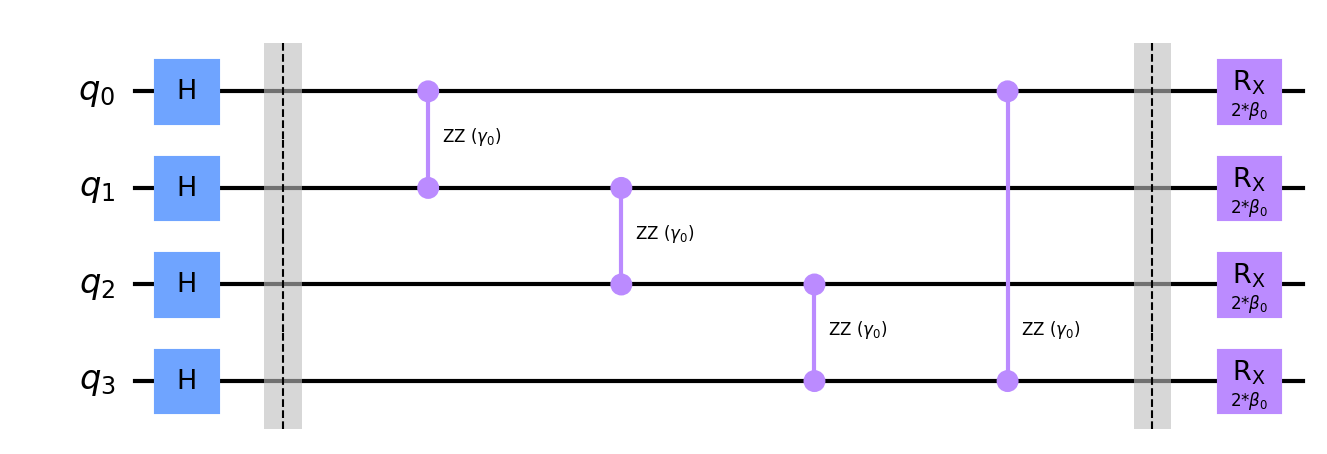
\includegraphics[scale=0.6]{circuits/qiskit/qiskit-circuit-2gamma-p1}
\end{figure}

\begin{figure}[htbp]{fig:4-qiskit_tutorial_circuito}{ Circuito de ejemplo de la página web~\cite{qiskit_tutorial_antiguo} ($p=1$) }
  \centering
  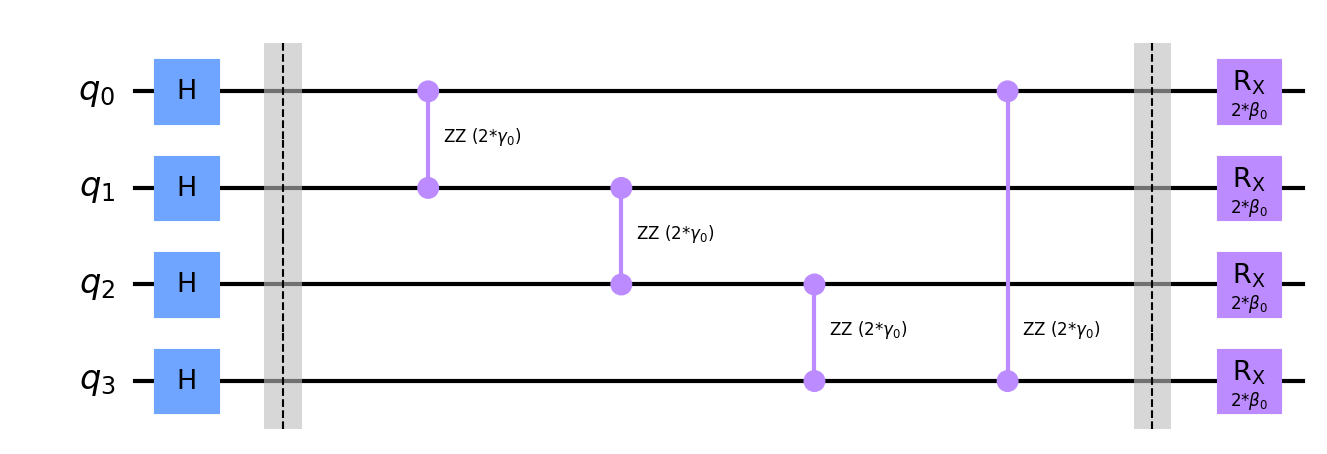
\includegraphics[scale=0.6]{circuits/qiskit/tutorial-qiskit-circuit-2gamma-p1}
\end{figure}

\paragraph{Diferencias con el circuito mostrado por Qiskit}

El circuito de ejemplo (\textit{Figura~\ref{fig:4-qiskit_tutorial_circuito}}) corresponde a desarrollar los mismos cálculos solo que con $f'(x) = 2*f(x)$. \\
Aunque las puertas \textit{Rzz} tengan coeficientes distintos ambas son correctas. Esto es porque ambos circuitos resultantes tienen un mismo estado fundamental, solo que uno lo tiene con el doble de energía que el otro. En otras palabras ambas funciones $f'$ y $f$ tienen un mismo $x$ que las minimiza.


%%% Local Variables:
%%% mode: latex
%%% TeX-master: "../tfgtfmthesisuam"
%%% End:
